\documentclass[10pt]{article}
\usepackage[a4paper,margin=1.45cm,top=1.3cm,bottom=1.5cm]{geometry}
\usepackage[T1]{fontenc}
\usepackage{lmodern}
\usepackage{microtype}
\usepackage{booktabs}
\usepackage{graphicx}
\usepackage{xcolor}
\usepackage{enumitem}
\usepackage{caption}
\usepackage{float}
\usepackage[hidelinks]{hyperref}
\setlist{nosep,leftmargin=1.2em}
\setlength{\parskip}{2.5pt}
\setlength{\parindent}{0pt}
\captionsetup{font=small,labelfont=bf,skip=3pt}
\newcommand{\sect}[1]{\vspace{3pt}{\large\bfseries #1}\par\vspace{1pt}}
\newcommand{\good}[1]{\textbf{#1}}

\begin{document}
\pagestyle{plain}

{\LARGE\bfseries Hand tracking for the V2D Track 3 pipeline: benchmark, experiments, results}\\[2pt]
{\small Ego2Sim team, 30 Oct 2026 (first version 29 Oct). Branch \texttt{pbasq/handbench}; code, numbers and videos in
\texttt{handtracking/} of the repo.}

\sect{Summary}
Track 3 has no ground truth for hands, so we built a benchmark that uses the two extra head cameras as judges, and then
tested fixes to the hand stage of our pipeline. The main finding is simple: \good{the baseline's hands are in the right
place in the image but about 26\,cm too far from the camera} (1.5$\times$ the true distance), because their depth comes
from a single-image depth network (MoGe). Rescaling each hand about the camera so it matches stereo depth fixes this:
3D joint error against our reference drops from \good{263\,mm to 50\,mm} without changing the image fit. One hand size per
hand and light temporal smoothing then make the tracks \good{5$\times$ smoother} at the same accuracy. A newer hand model
(HaWoR) and a learned stereo network (FoundationStereo) did not beat this. In simulation our new hands perform about the
same as the team's current hands.

We then tested on HOT3D, a public dataset filmed with Aria glasses with true hand positions from motion capture
(Section~5). (1) Our reference joints are themselves about 20\,mm from the true joints, so of our best method's 50\,mm,
roughly \good{39--46\,mm is real error}. (2) The stereo correction only helps when the stereo depth is good; on Aria's
cameras it made hands worse. (3) Moving HaWoR's hands onto the joints triangulated from all three cameras cut its error
against the true hands from \good{28\,mm to 22\,mm}: the most promising next step for Track 3.

\sect{1. How we evaluate (the benchmark)}
\textbf{The idea.} The head rig has three cameras side by side: \texttt{cam\_c} (left, mono), \texttt{cam\_a} (centre,
colour) and \texttt{cam\_b} (right, mono), about 3.7\,cm apart (Fig.~A1). Every method may only use \texttt{cam\_a}, like
the real pipeline's hand stage. \texttt{cam\_b} and \texttt{cam\_c} see the same hands from slightly different positions
and act as judges, the same way your two eyes judge distance.

\textbf{The reference (``pseudo ground truth'', Fig.~A7).} In each camera separately, a 2D hand-keypoint detector
(RTMPose) finds 21 hand joints on a zoomed crop of that camera's own image. For each joint seen confidently by
\texttt{cam\_a} and at least one judge camera, we draw a line from each camera through the point where it saw the joint,
and take the place where the lines cross as the joint's 3D position (triangulation). We keep the point only if, drawn back
into every camera used, it lands within 3 pixels of that camera's detection. A camera's keypoints for a hand are dropped
when most of them fall outside that hand's mask; this caught the detector jumping to the other hand when the hands are
close (Fig.~A6). The reference joints agree with stereo depth at the same pixels to 0.4\,mm (median); both come from the
same cameras, so this shows consistency, not accuracy (Section~5 measures accuracy).

\textbf{What we measure} (only on frames where the hand is visible in \texttt{cam\_a}, about 9{,}950 hand-frames over
the 20 public episodes; frames a method fills in by interpolation are never scored):
\begin{itemize}
\item \textbf{3D joint error} (mm): average distance between the method's joints and the reference joints. We split it
into \emph{depth} (error along the camera's line of sight: is the hand too near or too far?), \emph{lateral} (sideways
error) and \emph{pose} (error that remains after moving the method's hand onto the reference hand: wrong finger shape).
\item \textbf{Held-out camera check}: we take the method's 3D hand, which was built from \texttt{cam\_a} alone, and draw it
into \texttt{cam\_b}'s image. If the hand is in the right place in 3D, its joints should land where the keypoint detector
finds the joints in \texttt{cam\_b}'s own image. We report the average distance in pixels between the two, and the share
of joints that are within 10 pixels (called PCK). We also measure how well the drawn hand outline overlaps \texttt{cam\_b}'s
hand mask from SAM2: overlap area divided by combined area (IoU; 1 is a perfect match).
\item \textbf{Fit to the input camera}: the same checks in \texttt{cam\_a}. \textbf{Smoothness}: jitter (average joint
acceleration) and how much bone lengths vary over time. \textbf{Coverage}: share of visible hand-frames where the method
gives a hand.
\end{itemize}
A method is \emph{promoted} if it lowers the 3D error and improves the \texttt{cam\_b} check, without making the
\texttt{cam\_a} fit more than 5\% worse. Methods that cover different frames are also compared on the 5{,}316 hand-frames
they all cover.

\textbf{For scale.} Hands are about 0.40\,m from the head camera; a finger is about 15\,mm wide, so a 50\,mm error is
roughly three finger widths, and 1\,px in \texttt{cam\_b} is about 0.7\,mm sideways at the hand.

\textbf{Limits to keep in mind.} (1) The judge cameras are close to \texttt{cam\_a}: a 2\,cm depth error moves the hand
only about 2\,px in \texttt{cam\_b}, so the \texttt{cam\_b} check mostly tests sideways placement; depth is judged by the
3D error. (2) The reference is not exact: from the HOT3D test (Section~5) we estimate its joints are about 21\,mm (15
to 24\,mm) from the true joints, about 8\,mm of it a fixed difference in where RTMPose and MANO put each joint. This
inflates every method's 3D error similarly, and differences of a few mm between methods are not meaningful. (3) Methods that use stereo depth use \texttt{cam\_b}'s pixels as input; they are flagged below.
Getting the reference right also needed a re-calibration of the rig: the factory camera positions were 23--36\,px off on
the published videos; after refinement they are under 1\,px.

\sect{2. Experiments}
The models named below are explained, with pictures, in Fig.~A8: WiLoR finds the hands, HaMeR estimates a MANO hand
(a standard 3D hand model) in each frame, and HaWoR estimates MANO hands from a whole video clip.
\begin{table}[H]\small\centering
\begin{tabular}{@{}lp{0.655\linewidth}c@{}}
\toprule
ID & What it does & Uses stereo \\
\midrule
E0 & Baseline: cached upstream pipeline (WiLoR detection, SAM2 masks, HaMeR hand mesh, depth from MoGe, self-calibrated camera) & no \\
E0-refined & E0 + upstream's Gaussian-splat refinement & no \\
E1b-dz / -scale / -huber & Replace MoGe depth by SGBM stereo depth: slide along the view ray (upstream rule) / rescale about the camera / robust surface fit & yes \\
E1a, E1c, E1d & One hand size per hand; temporal smoothing (Savitzky--Golay, One-Euro, trajectory fit pulled to \texttt{cam\_a} keypoints); left/right swap repair & yes \\
\textbf{E1best-sgbm} & E1b-scale + one hand size per hand + Savitzky--Golay smoothing & yes \\
*-fs & Same as above with FoundationStereo (learned stereo network) instead of SGBM & yes \\
E2 HaWoR & HaWoR (CVPR 2025): end to end with its own camera tracking; and with our stereo rescaling & no / yes \\
E3 EgoFound3R & Skipped: its backbone weights (VGGT-Omega) are gated by Meta & -- \\
\bottomrule
\end{tabular}
\end{table}

\begin{table}[H]\small\centering
\begin{minipage}{\linewidth}\raggedright\sect{3. Results on Track 3}\end{minipage}\\[2pt]
\setlength{\tabcolsep}{3.9pt}
\begin{tabular}{@{}lccccccccc@{}}
\toprule
& 3D error & depth bias & lateral & pose & \texttt{cam\_b} kp (PCK) & \texttt{cam\_b} IoU & \texttt{cam\_a} kp & jitter & coverage \\
& mm & mm & mm & mm & px & & px & m/s$^2$ & \\
\midrule
E0 (baseline) & 263.4 & +259.6 & 26.4 & 42.4 & 25.3 (14\%) & 0.363 & 42.2 & 13.4 & 100\% \\
E0-refined & 262.3 & +256.5 & 31.3 & 42.2 & 30.2 (13\%) & 0.347 & 53.5 & 12.6 & 100\% \\
E1b-dz (stereo, upstream rule) & 58.2 & +21.9 & 23.6 & 42.5 & 26.1 (13\%) & 0.355 & 54.6 & 8.4 & 100\% \\
E1b-scale & 49.7 & +6.7 & 17.5 & 36.6 & 21.2 (23\%) & 0.410 & 42.0 & 7.8 & 100\% \\
\textbf{E1best-sgbm} & \textbf{49.5} & +6.7 & 17.3 & 36.5 & \textbf{21.0} (24\%) & 0.412 & 41.6 & \textbf{2.7} & 100\% \\
E1best-fs (FoundationStereo) & 49.8 & +3.7 & 17.2 & 36.5 & 21.0 (24\%) & 0.412 & 41.6 & 3.5 & 100\% \\
E1c-traj (pulled to \texttt{cam\_a} kps) & 55.4 & $-$1.4 & \textbf{12.2} & 36.6 & 17.9 (32\%)$^\dagger$ & 0.439 & 30.7$^\dagger$ & 11.5 & 100\% \\
E2 HaWoR (end to end) & 121.1 & +109.3 & 21.6 & 36.3 & 28.5 (21\%) & 0.415 & 44.7 & 9.9 & 94\% \\
E2 HaWoR + stereo & 53.2 & +15.8 & 19.1 & \textbf{34.9} & 26.5 (25\%) & \textbf{0.438} & 44.9 & 4.1 & 94\% \\
\bottomrule
\end{tabular}
\caption*{Each method on its own scored frames (all 20 episodes), errors against our reference joints. $^\dagger$E1c-traj
is fitted to the same \texttt{cam\_a} detector that builds the reference, so its keypoint scores are flattered. On the
5{,}316 common frames, HaWoR + stereo has the best \texttt{cam\_b} PCK (28\% vs 25\%) and \texttt{cam\_a} fit (IoU
0.301 vs 0.279), E1best-sgbm the best 3D error (49.3 vs 53.2\,mm). Full table: Table~A1.}
\end{table}
\vspace{-6pt}
\begin{enumerate}[leftmargin=1.4em]
\item \textbf{The baseline's problem is distance, not hand shape.} E0 places hands on average 26\,cm too far (1.5$\times$)
and inflates them by up to 25\% so they still match the image; in the image they look right (Fig.~A5), in 3D they float
behind the real hand (Fig.~A3). The cause is MoGe's depth scale: inside the hand masks it reads 1.45$\times$ the stereo
depth. This agrees with the team's earlier finding, against motion capture, that these reconstructions are 1.2--2.1$\times$
too large. The worst episodes are 39 (383\,mm; hands often leave the view), 24 (316\,mm; the largest MoGe scale, 1.61)
and 23 (316\,mm; an outlier focal-length estimate).
\item \textbf{How the depth is corrected matters.} Sliding the hand along its viewing ray to the stereo depth (the
upstream rule, E1b-dz) keeps the inflated size, so the hand looks too big and the image fit gets 25\% worse. Rescaling the
whole hand about the camera (E1b-scale) moves it closer and shrinks it by the same factor, so the image fit is unchanged
and depth bias drops to +7\,mm. Result: 3D error 81\% lower, \texttt{cam\_b} PCK from 14\% to 23\%.
\item \textbf{A stable size and smoothing cost no accuracy.} Rescaling every frame separately made the hand size flicker;
one size per hand (E1a) fixes that, and Savitzky--Golay smoothing removes jitter. E1best-sgbm is as accurate as E1b-scale,
5$\times$ smoother than E0, and its bone lengths vary by only 1.0\,mm.
\item \textbf{HaWoR has a better hand pose but worse depth here.} On its own it puts hands 11\,cm too far on Track 3
(on HOT3D its depth is good, Section~5) and misses 6\% of visible frames. With our stereo rescaling it is close to E1best
(53 vs 50\,mm) and has the best pose, mask overlap and \texttt{cam\_b} PCK, but a larger depth bias (+16 vs +7\,mm);
E1best's smoothing also makes it steadier (jitter 2.7 vs 4.1). Neither is better on every measure.
\item \textbf{A better stereo network did not help.} FoundationStereo gives depth for more of the hand (72\% vs 60\% of
mask pixels) but is not more accurate at the joints, and the methods built on it score the same. Swapping the depth source
leaves the remaining depth error unchanged, so that error does not come from stereo noise.
\item \textbf{In simulation (teammate's replay, 9 episodes, same camera, objects and retargeting for both):} our
E1best-sgbm hands perform about the same as the team's current hands (Rian's \texttt{objfill\_v2s}). Medians over the 9
episodes: gap between fingertips and the object 1.05 vs 0.90\,cm; fingertips touching the object while it moves 93\% vs
92\% of the time; the team's robot hands keep contact more often (84\% vs 73\%). In episode 40 both grip the dustpan the
same way; in episode 41 our right hand hovers next to the pan handle while the team's grips it (Fig.~A4). The team's hands
fill in grasps using the object's position, and ours are about 15\% too big in simulation because the loader ignores our
per-hand size factor.
\end{enumerate}

\sect{4. Discussion}
For this rig, the biggest lever is where the hand's distance comes from: metric stereo beats single-image depth by an
order of magnitude, as long as the correction keeps the hand matching the image. The remaining $\sim$50\,mm against our
reference splits into hand position (31\,mm, of which 24\,mm is along the viewing ray) and finger pose (35--37\,mm).
The first version of this report suggested that much of this was the reference's own error. The HOT3D test (Section~5)
shows that is only partly true: the reference adds about 20--26\,mm, and independent errors add like the sides of a
right-angled triangle ($\sqrt{a^2+b^2}$), so our best method's true error is about 39--46\,mm. Most of the remaining
error is real, and better stereo does not reduce it. For the robot, grasp handling and hand size in the simulation chain
matter as much as camera-frame accuracy.

\sect{5. Checks against true hand positions (HOT3D)}
\textbf{The data.} HOT3D is a public dataset of people handling objects, filmed with Aria glasses: one colour camera and
two mono cameras, like our rig, plus true 3D hands from motion-capture markers, stored as MANO hands. We used 8 clips of
150 frames (Fig.~A9; licence: non-commercial research only). The Aria cameras are laid out differently from ours: the
colour camera sits only 1.5\,cm from the left mono camera and about 13\,cm from the right one, while all our camera pairs
are 3.7--7.5\,cm apart.

\textbf{Why HaWoR stands in for HaMeR.} On Track 3, E1best's hands come from the upstream pipeline's cached HaMeR run,
and we only add the depth correction and smoothing. We could not run the upstream HaMeR stage on HOT3D, so there the hands
come from HaWoR and we apply our steps to them. These tests check our correction steps, not E1best's exact hands.

\begin{table}[H]\small\centering
\setlength{\tabcolsep}{4pt}
\begin{tabular}{@{}lccc@{}}
\toprule
Hands, compared with the true hands (7 clips, 1{,}433 hand-frames) & 3D error, mean (median) & depth bias & jitter \\
& mm & mm & m/s$^2$ \\
\midrule
HaWoR, raw & 28.4 (22.7) & $-$17.0 & 8.2 \\
HaWoR + our Track 3 recipe (E1best steps: stereo rescale, one size, smoothing) & 128.5 (48.2) & +68.2 & 29.9 \\
HaWoR + one stereo scale per hand per clip + smoothing & 84.4 (34.9) & +44.8 & 3.7 \\
HaWoR moved onto the triangulated joints, in the frames that have them & 25.9 (19.6) & $-$12.7 & 14.2 \\
\quad + the same move carried across frames without them (up to 30 frames) & 22.3 (16.3) & $-$3.4 & 9.8 \\
\quad + stereo where nothing else applies, + smoothing & \textbf{21.6 (15.8)} & \textbf{$-$3.2} & \textbf{3.6} \\
\bottomrule
\end{tabular}
\end{table}
\vspace{-4pt}
\begin{enumerate}[leftmargin=1.4em]
\item \textbf{Stereo correction only helps when the stereo is good.} Applied to HaWoR on HOT3D, our Track 3 recipe made the
hands much worse (28 to 129\,mm). Aria's mono cameras give stereo depth for only 12--17\% of the pixels at the hand joints
(67\% on our rig), and for left hands that depth reads 30--80\% too far. HaWoR's own depth was already good on HOT3D, while
on Track 3 it was 11\,cm off. So whether a stereo correction helps depends on both the footage and the stereo quality; a
pipeline should check the stereo for each hand (enough valid pixels, stable over time) before using it.
\item \textbf{How accurate our reference is (``measuring the floor'').} We rebuilt the reference on HOT3D with exactly the
Track 3 steps and compared its joints with the true joints. Where the camera pair is well spread (all three cameras, or
colour + right mono), the reference joints are 19\,mm (mean) and 15\,mm (median) from the true joints; joints from the
1.5\,cm pair are useless (96\,mm) and must be left out. About 8\,mm of the error is a fixed offset per joint: MANO's joints
sit inside the hand, on its skeleton, while the detector was trained on joints marked on the hand's surface. A simple model
of how keypoint error turns into depth error (it grows with distance squared and shrinks with camera spacing) matches
the HOT3D measurements; applied to our rig, it gives about 21\,mm (median, 15 to 24\,mm) for the Track 3 reference. This
is an estimate, as Track 3 has no hand ground truth. On the same HOT3D joints, HaWoR scored 33\,mm against the reference
and 26\,mm against the true hands; combining 26 and 19\,mm as in Section~4 gives exactly 33\,mm.
\item \textbf{Triangulated keypoints improve hands, even on Aria.} We used the triangulated joints, built only from HaWoR's
own hand outlines and never from the true hands, to correct HaWoR: in each frame with at least 4 well-placed joints, the
whole hand is moved (not rotated or rescaled) so its joints line up with the triangulated ones. The move is then carried
across frames without triangulated joints, because HaWoR's depth error changes slowly. Error against the true hands fell
from 28.4 to 21.6\,mm (median 22.7 to 15.8\,mm), the depth bias almost disappeared, and all 7 clips improved. In the 34\%
of frames with triangulated joints it fell from 22 to 14\,mm; carrying the move reached 76\% of frames, stereo only 1\%.
Also fitting a rotation and size to these few, noisy joints made results worse (27\,mm).
\end{enumerate}

\sect{6. Next steps} In rough order of value for effort:
\begin{enumerate}[leftmargin=1.4em]
\item \textbf{Use the triangulated keypoints inside the Track 3 method}: move E1best-sgbm's hands onto the triangulated
joints and carry the move across gaps, as on HOT3D; all our camera pairs are usable, so the gain should be larger. It
cannot be scored against the current reference, which uses the same joints. Instead, build it from \texttt{cam\_a} and
\texttt{cam\_b} only, and check it against the keypoints found in \texttt{cam\_c}, which it never used.
\item \textbf{Score the team's current hands (\texttt{objfill\_v2s}) on this benchmark}, so all hand sources are
compared on the same frames. Cheap, and it shows whether E1best is better before grasp filling or only equal.
\item \textbf{Fix hand size in the simulation chain}: pass our per-hand size into the loader (or fold it into the MANO
shape), and re-run the teammate's replay. Hands 15\% too big change where fingertips land on objects.
\item \textbf{Combine strengths}: E1best's depth with the team's object-aware filling of grasps; and pick E1best or
HaWoR + stereo frame by frame, with a small model predicting which is more reliable (planned E4/E5).
\item \textbf{Hand-label 60 frames in two cameras} (3--4 hours) to measure the reference's error on our own rig.
\end{enumerate}

%% ------------------------------------------------------------------------------------------------ appendix
\clearpage
\section*{Appendix: figures and full results}
\begin{figure}[H]\centering
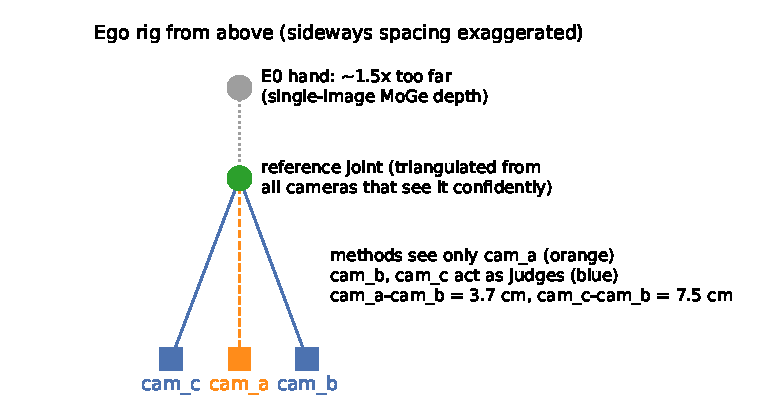
\includegraphics[width=0.48\linewidth]{figs/fig_rig.pdf}\hfill
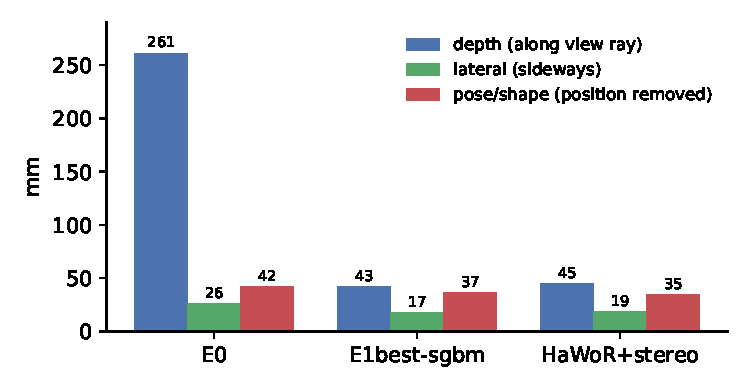
\includegraphics[width=0.47\linewidth]{figs/fig_error_parts.pdf}
\caption*{\textbf{Fig.~A1.} Left: the benchmark idea. Methods see only \texttt{cam\_a}; reference joints are triangulated
from all cameras that see the joint confidently. Right: where the 3D error comes from, for the baseline, our best method
and HaWoR + stereo. E0's error is almost all depth; after the stereo correction, depth, sideways and finger-pose errors
are of similar size.}
\end{figure}
\begin{figure}[H]\centering
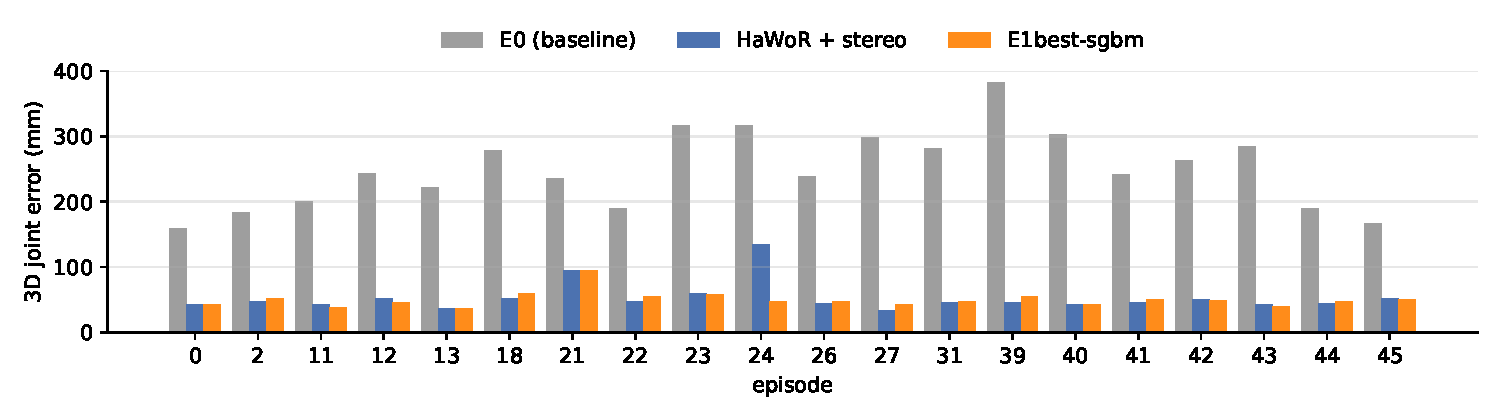
\includegraphics[width=\linewidth]{figs/fig_per_episode.pdf}
\caption*{\textbf{Fig.~A2.} 3D joint error per episode. The stereo correction helps every episode; episode 21 (watering
can, hands often occluded) remains the hardest, and HaWoR fails on episode 24.}
\end{figure}
\begin{figure}[H]\centering
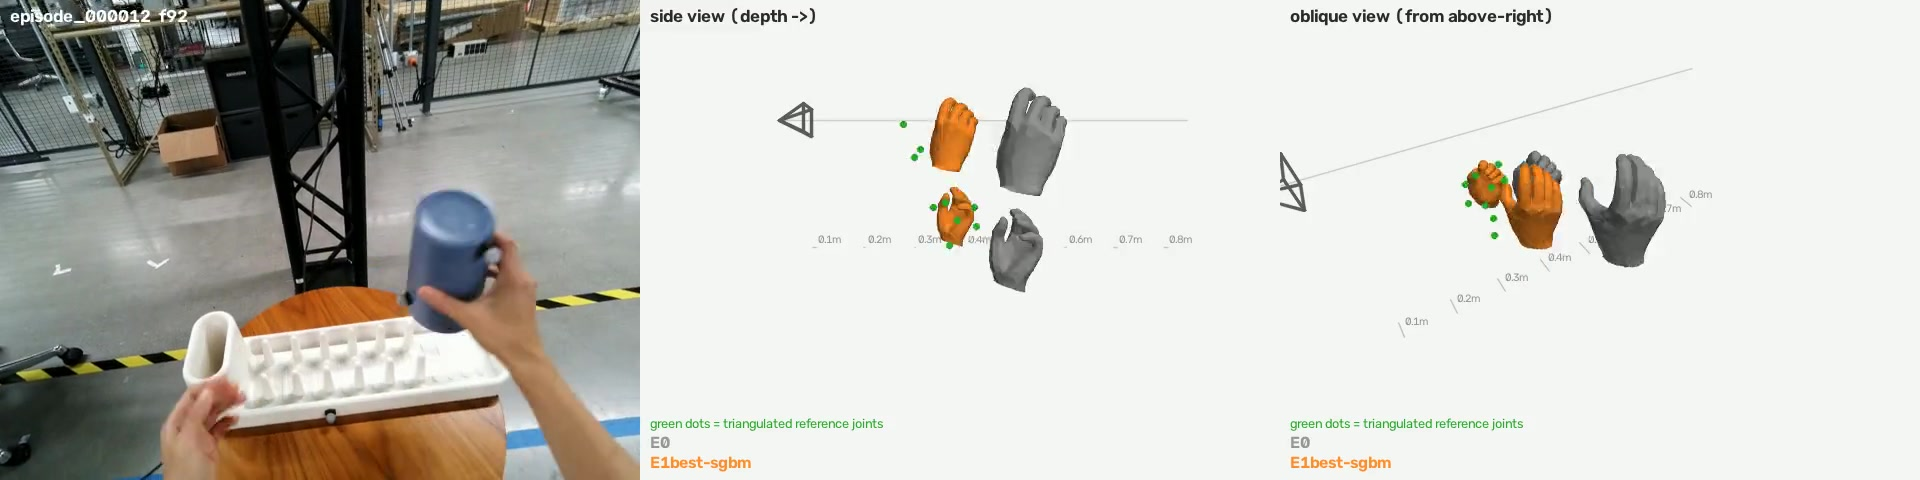
\includegraphics[width=\linewidth]{figs/fig_3d_ep12.jpg}\\[2pt]
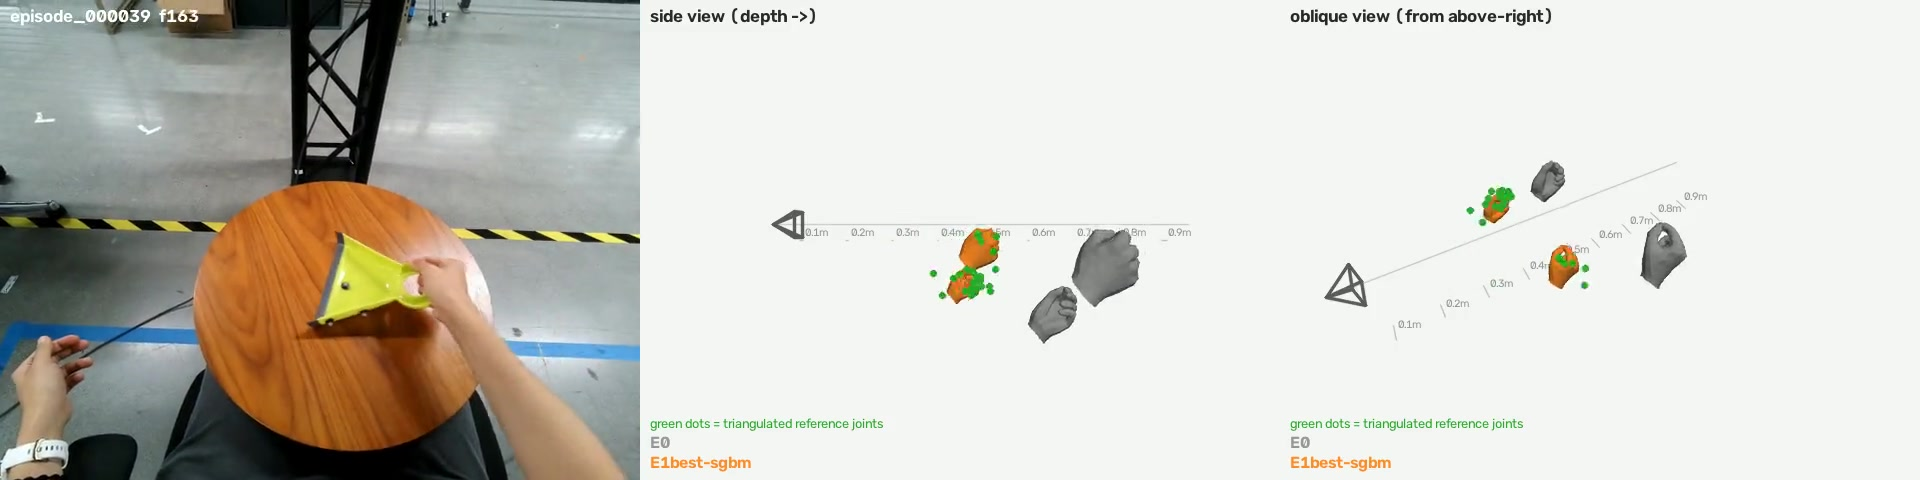
\includegraphics[width=\linewidth]{figs/fig_3d_ep39.jpg}
\caption*{\textbf{Fig.~A3.} The same moment seen from beside the head (middle) and from above-right (right), episodes 12
and 39. Grey = E0, orange = E1best-sgbm, green dots = reference joints, triangle = head camera, ticks every 10\,cm of
depth. E0's hands float 15--35\,cm behind the reference and are too big; E1best's sit on it.}
\end{figure}
\begin{figure}[H]\centering
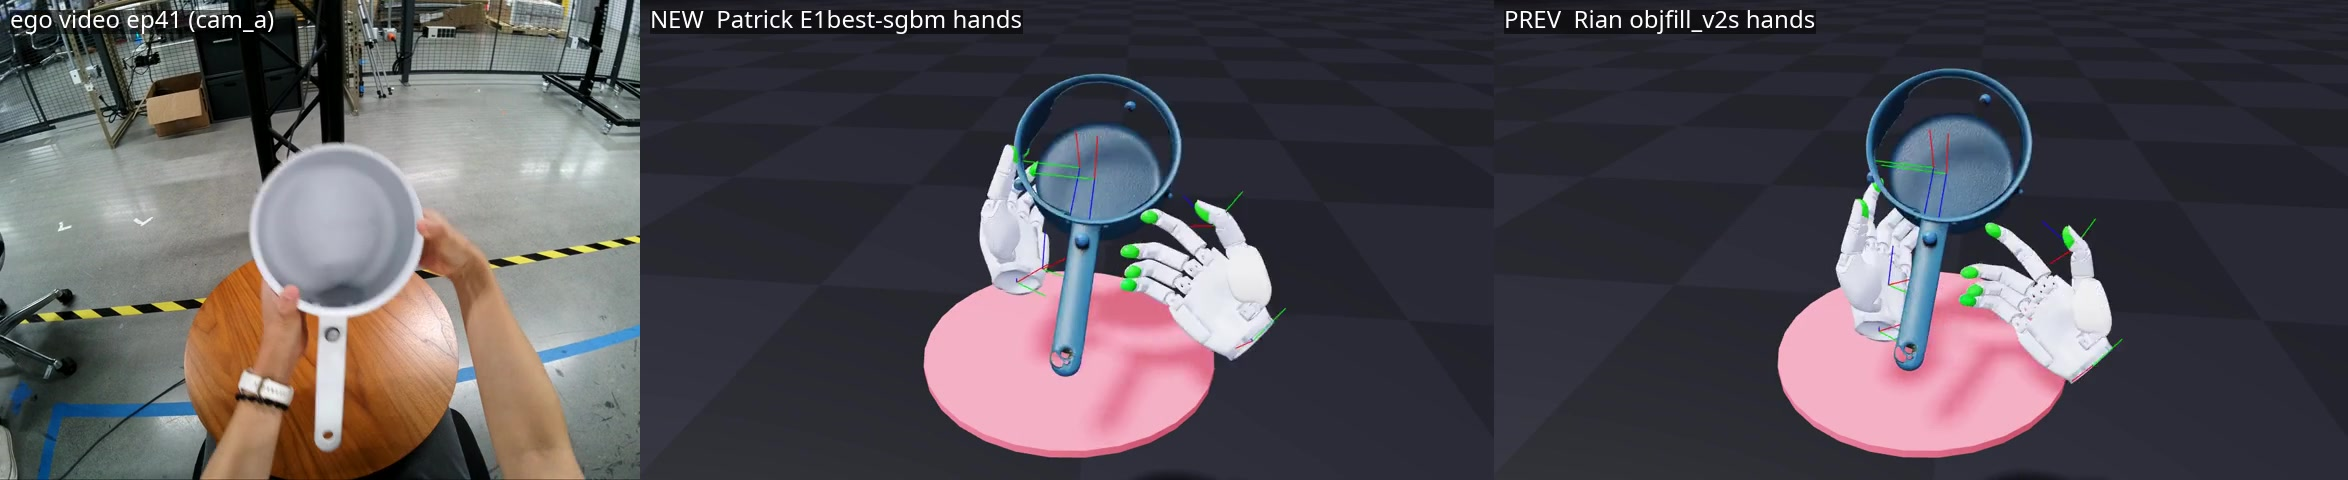
\includegraphics[width=\linewidth]{figs/fig_sim_ep41.jpg}\\[2pt]
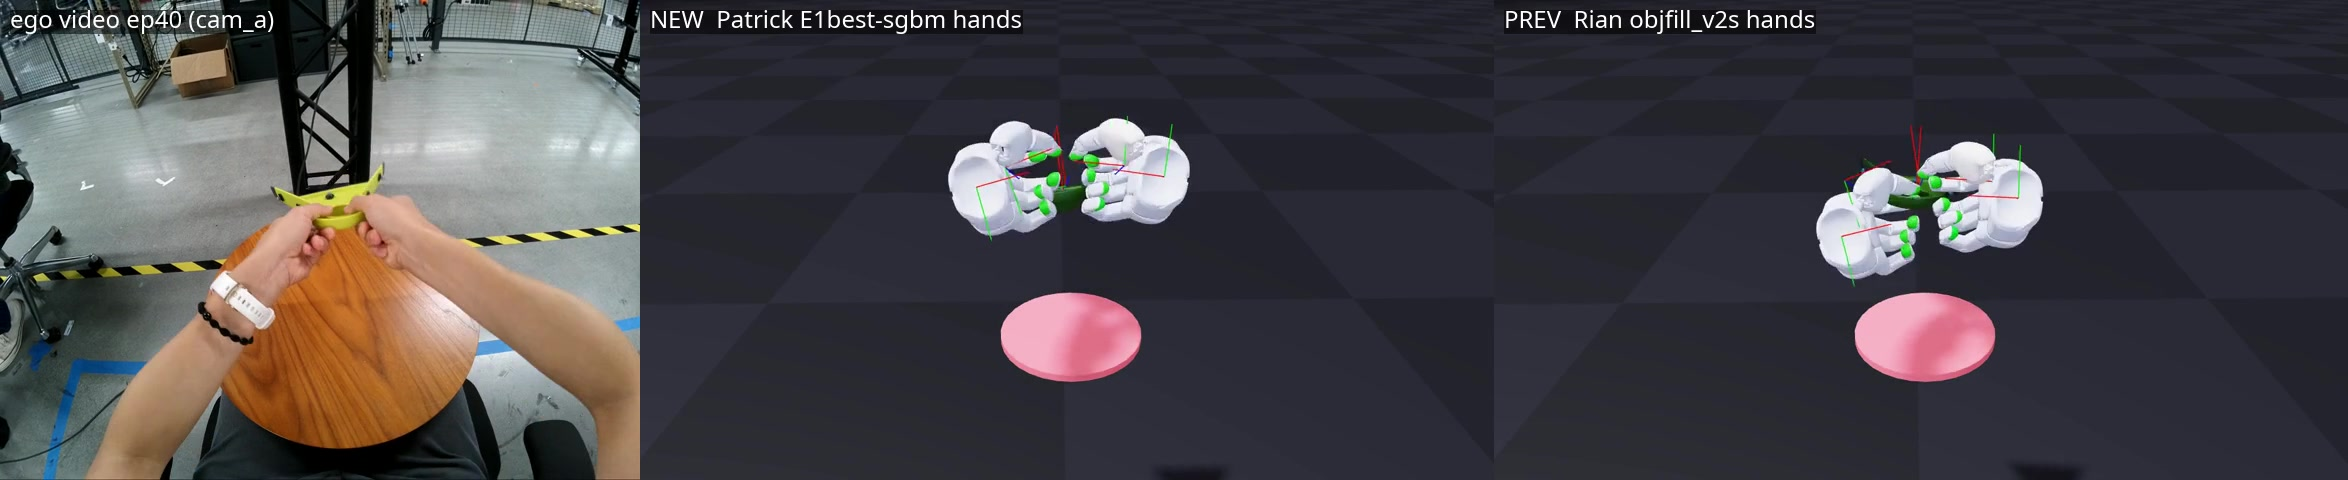
\includegraphics[width=\linewidth]{figs/fig_sim_ep40.jpg}\\[2pt]
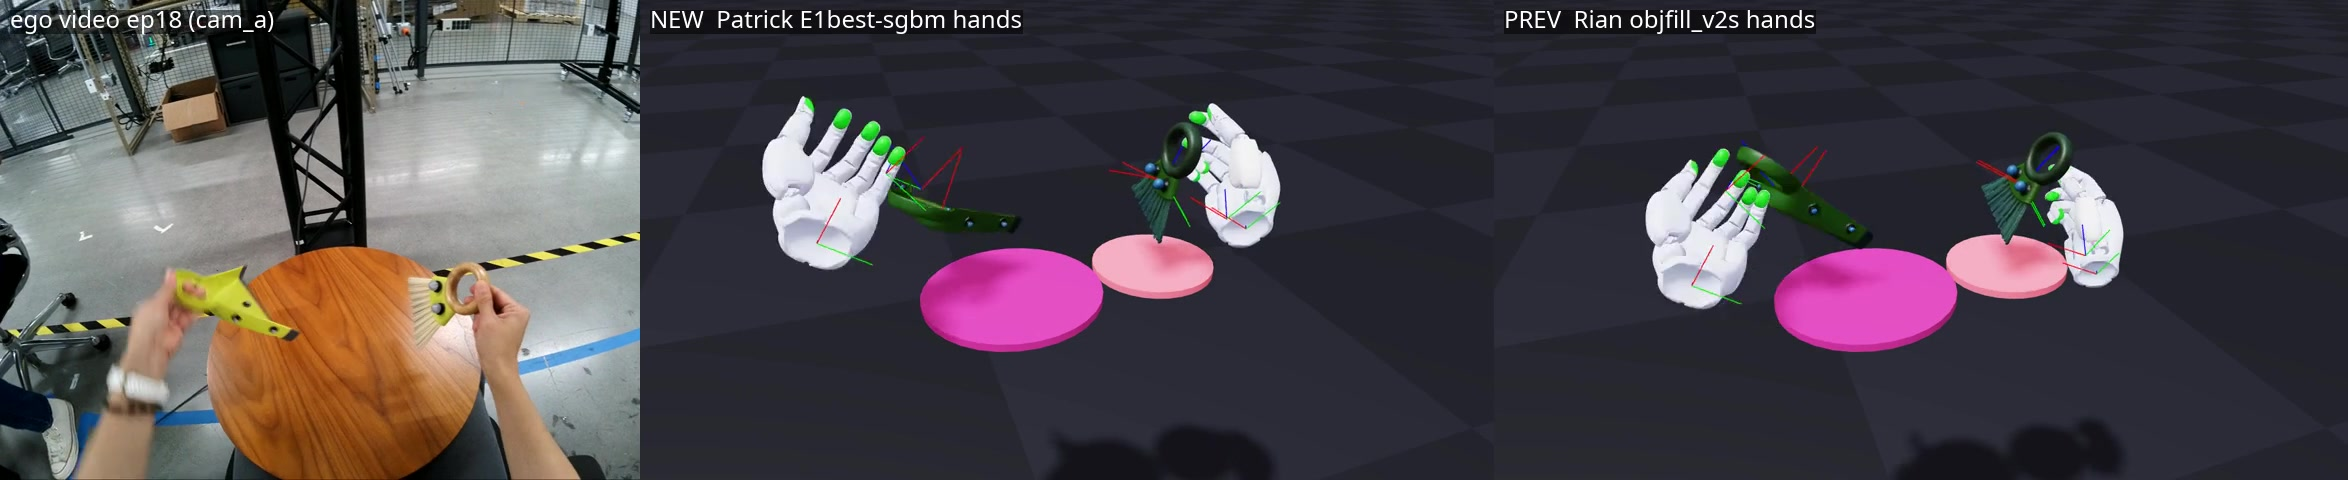
\includegraphics[width=\linewidth]{figs/fig_sim_ep18.jpg}
\caption*{\textbf{Fig.~A4.} Teammate's physics replay in FlashCHORD (Sharpa hands, ground-truth objects): ego video | new
(E1best-sgbm) | previous team hands (\texttt{objfill\_v2s}). Episode 41: our right hand hovers beside the handle while the
team's grips it. Episode 40: same grip. Episode 18: comparable.
Videos: \texttt{v2d\_challenge\_data/outputs/handtracking\_sim\_compare/videos/}.}
\end{figure}
\begin{figure}[H]\centering
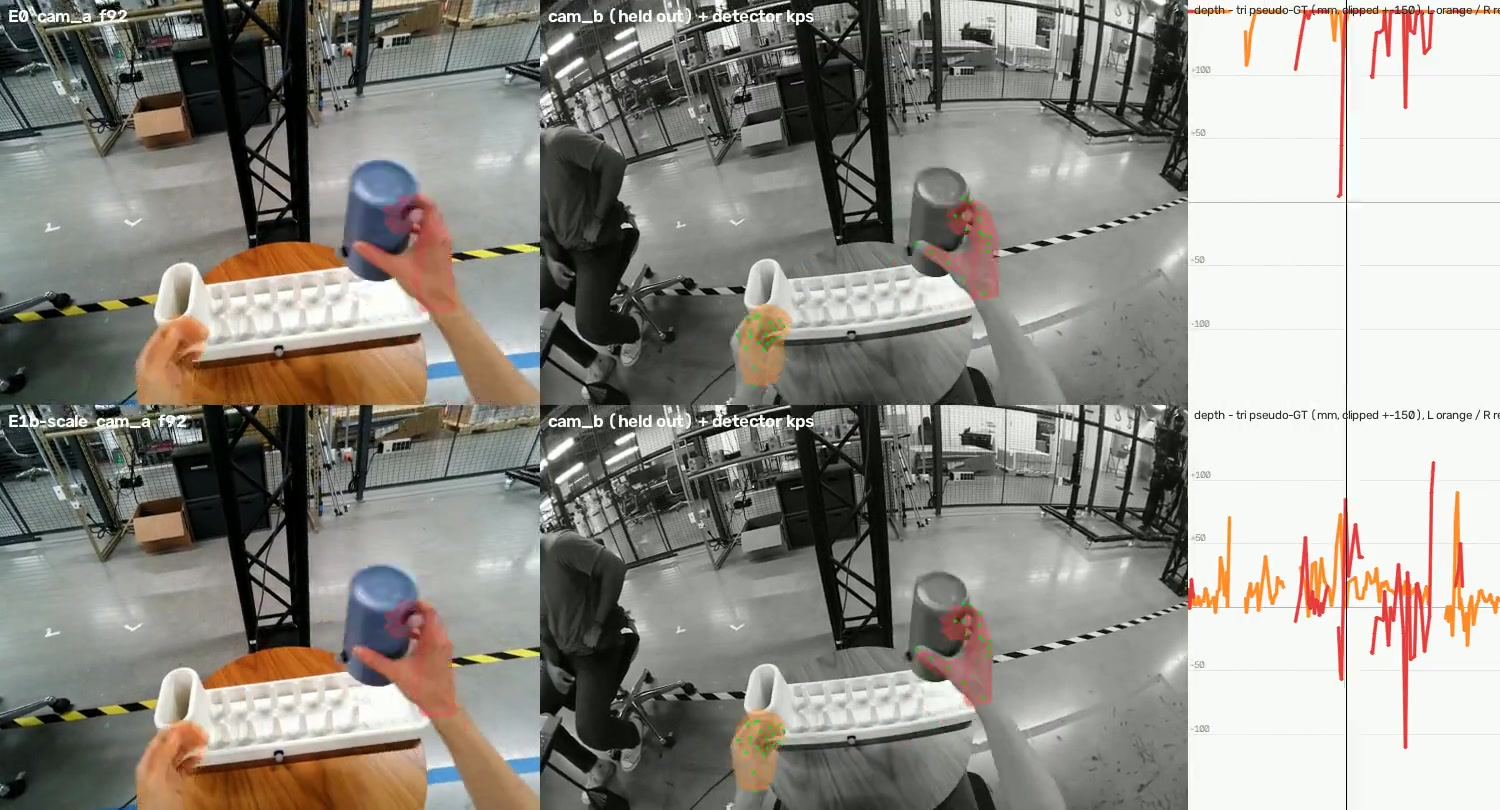
\includegraphics[width=\linewidth]{figs/fig_overlay_ep12.jpg}
\caption*{\textbf{Fig.~A5.} Why 2D views hide the problem. Top: E0; bottom: E1b-scale (same hand shapes, corrected depth).
Left: \texttt{cam\_a} input with meshes. Middle: held-out \texttt{cam\_b} with the meshes drawn in and \texttt{cam\_b}'s
own keypoints (green). Right: depth error against the reference over the episode (clipped at $\pm$150\,mm): E0 sits above
+150\,mm throughout, E1b-scale stays near zero. In both image views the hands look roughly right.}
\end{figure}
\begin{figure}[H]\centering
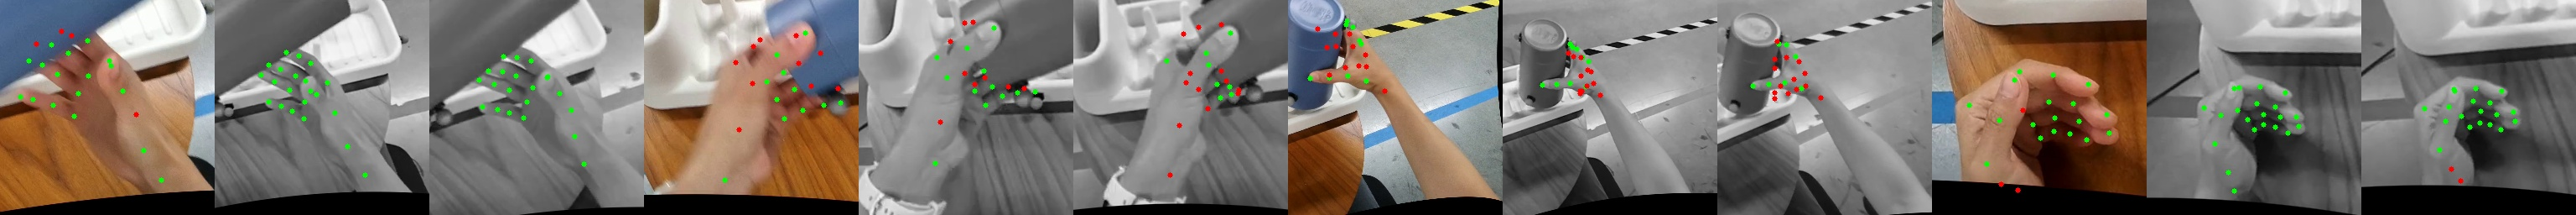
\includegraphics[width=\linewidth]{figs/fig_crops.jpg}\\[3pt]
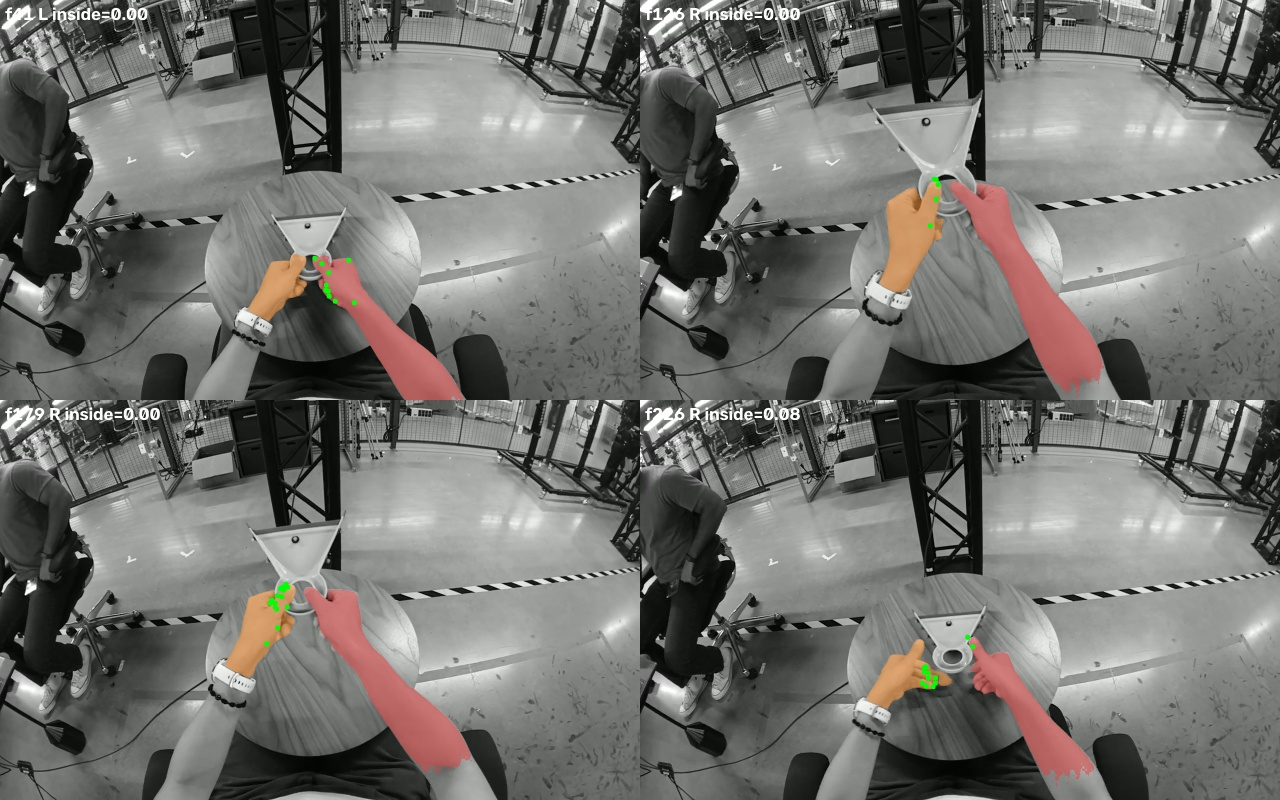
\includegraphics[width=0.49\linewidth]{figs/fig_gate_ep40.jpg}\hfill
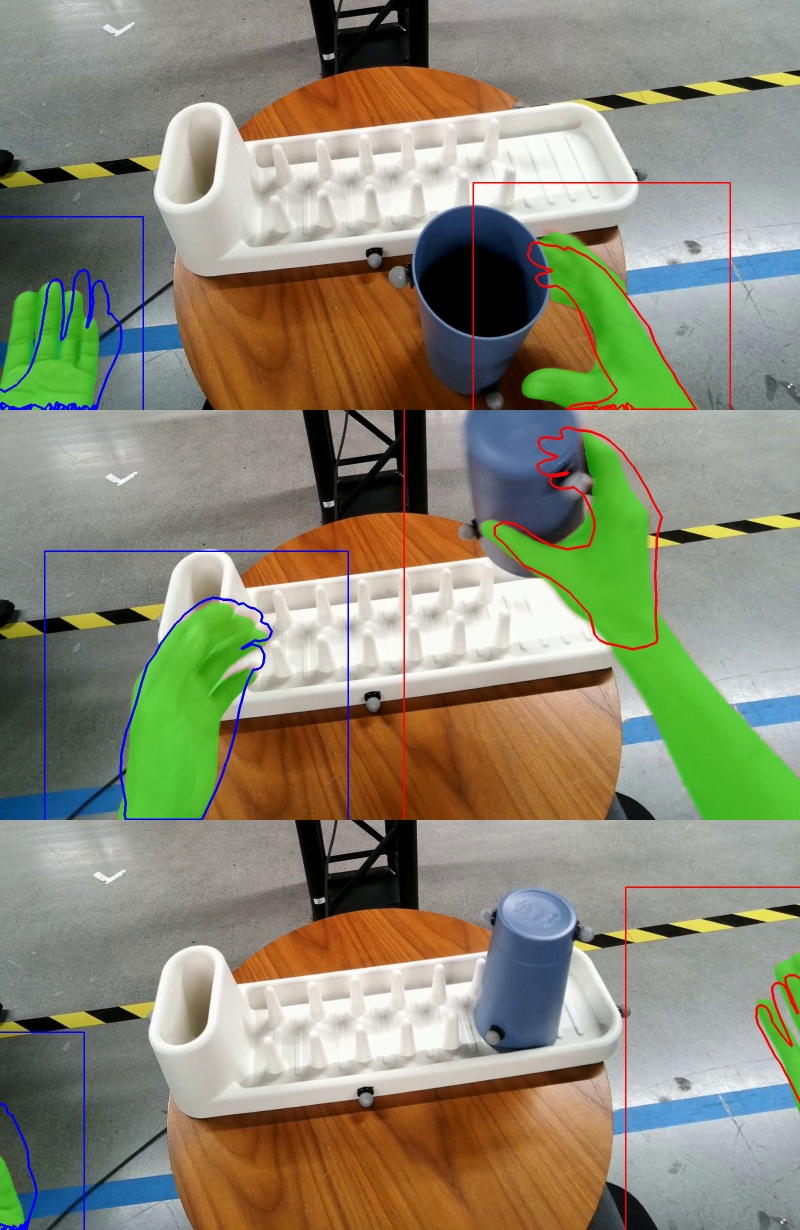
\includegraphics[width=0.36\linewidth]{figs/fig_forearm_masks.jpg}
\caption*{\textbf{Fig.~A6.} Building the reference. Top: zoomed crops of the same hands in \texttt{cam\_a} (colour) and the
judge cameras (mono), with RTMPose keypoints (green = confident, red = not). Bottom left: what the mask check catches:
keypoints for the right hand (green) were detected on the left hand, although the masks are correct; such views are
dropped. Bottom right: SAM2 ``hand'' masks include the forearm, so mask overlap is measured only inside the hand region.}
\end{figure}
\begin{figure}[H]\centering
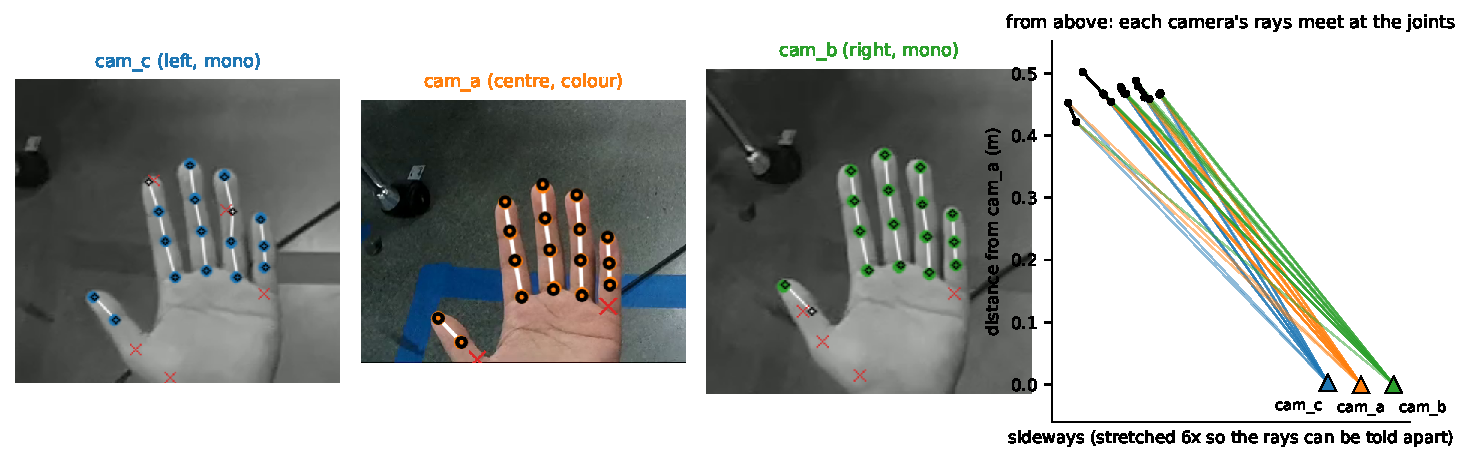
\includegraphics[width=\linewidth]{figs/fig_triangulation.pdf}
\caption*{\textbf{Fig.~A7.} How one reference hand is built (episode 12, frame 2, left hand). Left three panels: the same
hand in each camera. Coloured dots are the RTMPose keypoints that were used; red crosses are confident keypoints that were
rejected because they did not agree with the other cameras within 3 pixels; black rings joined by white lines are the
final 3D reference joints drawn back into that camera. Right: the same hand seen from above. Each line runs from a camera
through the place where that camera saw a joint, and the joint is placed where the lines meet. The sideways direction is
stretched 6 times, because the cameras are only 3.7\,cm apart and the lines would otherwise lie on top of each other.
Joints seen by all three cameras are the most reliable; joints seen by \texttt{cam\_a} and one other camera are kept too.}
\end{figure}
\begin{figure}[H]\centering
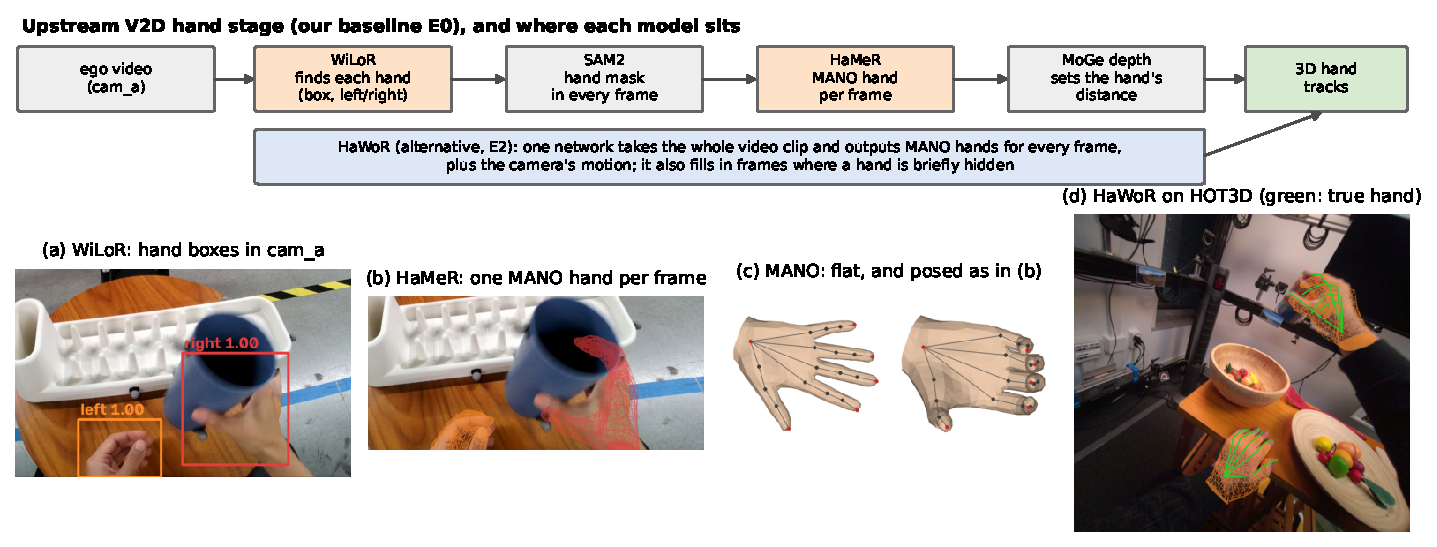
\includegraphics[width=\linewidth]{figs/fig_models.pdf}
\caption*{\textbf{Fig.~A8.} The hand models named in this report, and where they sit in the upstream V2D hand stage (top).
\textbf{(a) WiLoR} is a hand detector: it finds each hand in the image, draws a box around it and says whether it is a left
or right hand (score 1.00 = certain). Its boxes start the SAM2 hand masks. WiLoR can also output a hand mesh, but in the
upstream run we use (E0) the meshes come from HaMeR. \textbf{(b) HaMeR} looks at one image crop around a detected hand and outputs a MANO hand for
that frame (red: the right hand in E0, episode 12, frame 40). It cannot judge well how far away the hand is, which is why
upstream takes the distance from MoGe depth and we take it from stereo. \textbf{(c) MANO} is not a network but a fixed
3D hand model: a mesh of 778 points with 21 joints (dots; red = wrist and fingertips), controlled by about 61 numbers:
10 for hand shape, 45 for finger bends and 6 for the wrist's position and rotation. Left: all finger bends at zero.
Right: the finger bends HaMeR estimated in (b). HaMeR, WiLoR, HaWoR and HOT3D's ground truth all describe hands as MANO
numbers, which is why their outputs can be compared joint by joint. \textbf{(d) HaWoR} takes a whole video clip instead of
single images, outputs a MANO hand for every frame together with the camera's motion, and fills in frames where a hand is
briefly hidden. Shown on HOT3D (orange) with the true hand from motion capture (green skeleton); in the image the two look
alike, and the difference is mostly in distance (see Fig.~A9, bottom right).}
\end{figure}
\begin{figure}[H]\centering
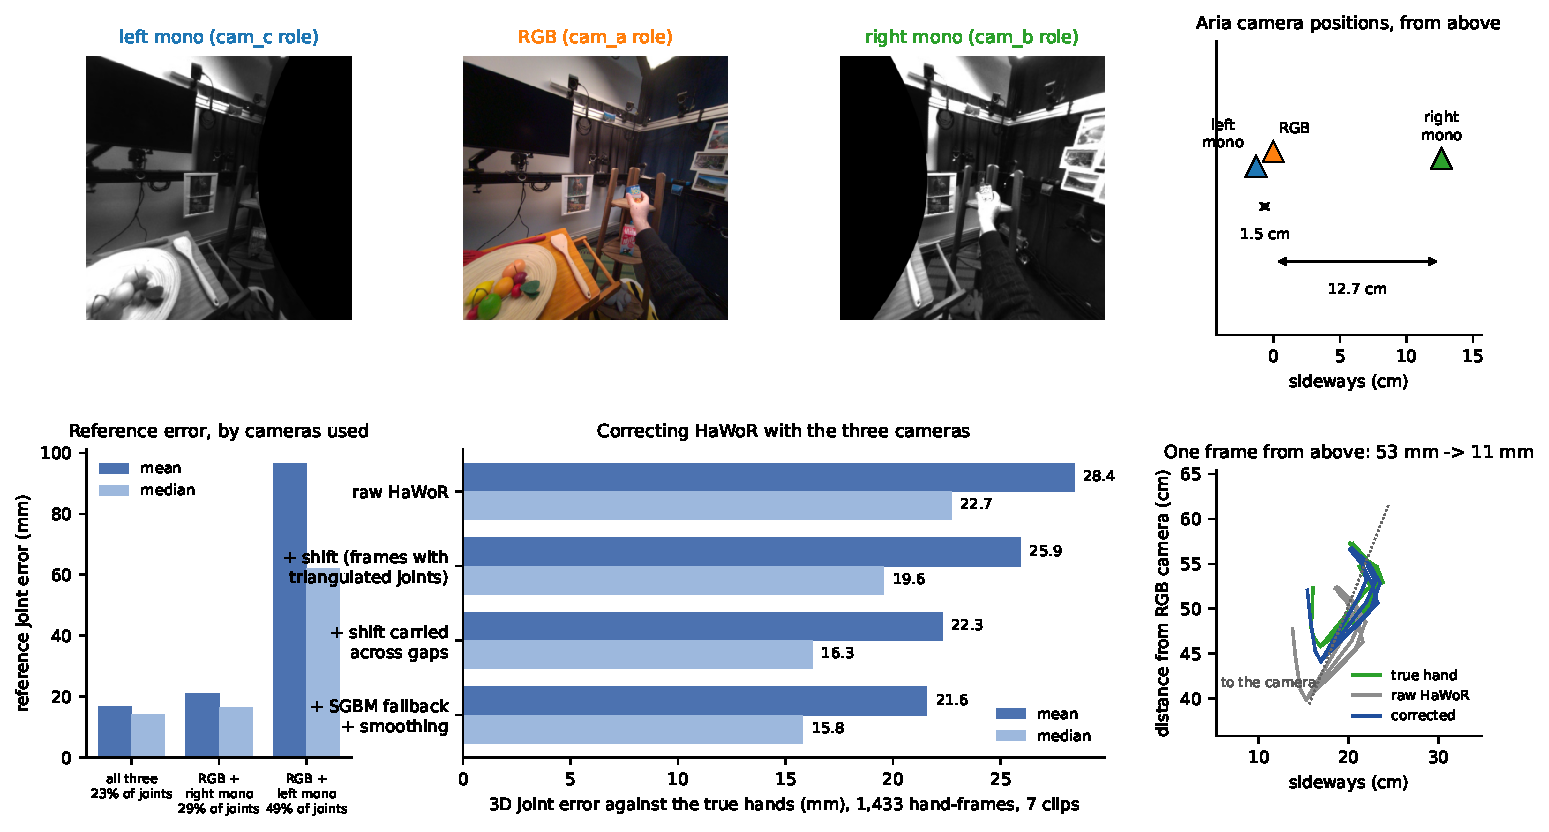
\includegraphics[width=\linewidth]{figs/fig_hot3d.pdf}
\caption*{\textbf{Fig.~A9.} The HOT3D tests (Section~5). Top: one frame from the three Aria cameras, each re-projected into
an ordinary pinhole view, and where the cameras sit on the glasses; we use them in the roles of \texttt{cam\_c},
\texttt{cam\_a} and \texttt{cam\_b}. Bottom left: how far the reference joints are from the true joints, by the cameras
that saw them; the 1.5\,cm pair is useless. Bottom middle: HaWoR's error against the true hands, step by step, as we move
its hands onto the triangulated joints. Bottom right: one frame from above (clip 003147, right hand, true scale): raw
HaWoR (grey) is 53\,mm from the true hand (green), mostly along the line to the camera; after the correction (blue) it is
11\,mm away.}
\end{figure}

\begin{table}[H]\small\centering
\setlength{\tabcolsep}{4pt}
\begin{tabular}{@{}lccccccccccc@{}}
\toprule
method & stereo & 3D err & depth & lateral & bias & pose & \texttt{cam\_b} kp & PCK & \texttt{cam\_b} IoU & jitter & bone std \\
\midrule
E0 & no & 263.4 & 261.3 & 26.4 & +259.6 & 42.4 & 25.3 & 14\% & 0.363 & 13.4 & 1.05 \\
E0-refined & no & 262.3 & 258.2 & 31.3 & +256.5 & 42.2 & 30.2 & 13\% & 0.347 & 12.6 & 1.93 \\
E1b-dz & yes & 58.2 & 48.5 & 23.6 & +21.9 & 42.5 & 26.1 & 13\% & 0.355 & 8.4 & 0.93 \\
E1b-scale & yes & 49.7 & 42.6 & 17.5 & +6.7 & 36.6 & 21.2 & 23\% & 0.410 & 7.8 & 3.69 \\
E1b-huber & yes & 49.7 & 42.6 & 17.6 & +6.2 & 36.7 & 21.5 & 23\% & 0.406 & 8.7 & 10.07 \\
E1a-size-dz & yes & 49.6 & 42.6 & 17.4 & +6.8 & 36.5 & 21.1 & 24\% & 0.413 & 8.5 & 0.11 \\
E1c-savgol & yes & 49.6 & 42.6 & 17.4 & +6.7 & 36.6 & 21.1 & 24\% & 0.410 & 2.6 & 3.56 \\
E1c-oneeuro & yes & 51.2 & 43.0 & 20.2 & +5.7 & 36.7 & 30.2 & 15\% & 0.356 & 2.3 & 3.42 \\
E1c-traj & yes & 55.4 & 51.6 & 12.2 & $-$1.4 & 36.6 & 17.9 & 32\% & 0.439 & 11.5 & 3.69 \\
E1best-sgbm & yes & 49.5 & 42.5 & 17.3 & +6.7 & 36.5 & 21.0 & 24\% & 0.412 & 2.7 & 0.99 \\
E1b-scale-fs & yes & 50.0 & 43.1 & 17.4 & +3.8 & 36.6 & 21.2 & 23\% & 0.411 & 10.5 & 4.61 \\
E1best-fs & yes & 49.8 & 42.9 & 17.2 & +3.7 & 36.5 & 21.0 & 24\% & 0.412 & 3.5 & 0.98 \\
E2-hawor & no & 121.1 & 115.3 & 21.6 & +109.3 & 36.3 & 28.5 & 21\% & 0.415 & 9.9 & 1.43 \\
E2-hawor + stereo & yes & 53.2 & 44.7 & 19.1 & +15.8 & 34.9 & 26.5 & 25\% & 0.438 & 4.1 & 2.05 \\
E2-hawor + stereo (fs) & yes & 52.8 & 44.3 & 19.0 & +12.8 & 34.9 & 26.4 & 25\% & 0.440 & 5.5 & 2.92 \\
\bottomrule
\end{tabular}
\caption*{\textbf{Table~A1.} All methods, own scored frames, 20 public episodes, errors against our reference joints
(E1a-betas and E1d-swaps were identical to E1b-scale and are omitted). Errors in mm, \texttt{cam\_b} keypoints in px, jitter
in m/s$^2$. HaWoR rows cover 94\% of visible hand-frames, all others 100\%.}
\end{table}
\end{document}
